\chapterstart{研究谱系与独立发现}
\label{sec:lineage}

三阶段研究同时产生了模型改进与独立科学发现。紧凑文本、残差模型和后续训练形成了两代模型的继承关系；围绕关系识别、信息读取与测量方法的探索，则发展出各有实验依据的研究分支。本章说明这些分支解决了什么问题、与主线怎样联系，以及能够供后续研究使用的认识和方法。

这些研究覆盖从文本进入模型、能力逐步形成，到后续学习和结果测量的多个层次。表\ref{tab:research_scope}按所解决的问题归纳其代表性产出；后文进一步解释经验替换、关系锚点、身份匹配和测量控制等发现。附录\ref{app:catalog}保留完整主题及其结论状态，配套材料提供相应的推导、程序、实验与研究笔记。

\begin{table}[htbp]
\caption{三阶段研究的主要问题与代表性产出。模型方法、机制认识和实验工具分别提供可继续使用的研究基础。}
\label{tab:research_scope}
\small
\begin{tabularx}{\linewidth}{@{}P{29mm}Y Y@{}}
\toprule 研究层次 & 具体问题 & 代表性产出\\\midrule
经验与数据组织 & 固定预算下，应如何选择内容、压缩表达和安排相关文本？ & 紧凑重述与预算再分配；固定预算替换；关系类型与预测窗口对照。\\
表示、结构与先验 & 文本怎样表示，少量监督如何确定关系并被新输入使用？ & 字符与子词比较；零初始化残差增量；稀疏锚点、共享表示和身份匹配。\\
学习信号与能力 & 哪些预测训练了关系使用，怎样检验计算是否真正参与回答？ & 输入与监督分离；关系监督分配；熟悉与未见符号对照及内部信号干预。\\
优化与学习动力学 & 数据价值如何随训练变化，新能力如何与原有功能共存？ & 早晚期轨迹、课程与优化器比较；关系经验剂量；增量学习与保持配置。\\
评测、归因与计算 & 怎样得到可解释的比较，并保证实现与所研究的方法一致？ & 共同参数初始化；来源隔离与逐题分析；完整模型加载、预算记账与梯度一致性检查。\\
\bottomrule
\end{tabularx}
\end{table}

\subsection{实践继承、问题深化与方法结合}

\begin{figure}[htbp]
\centering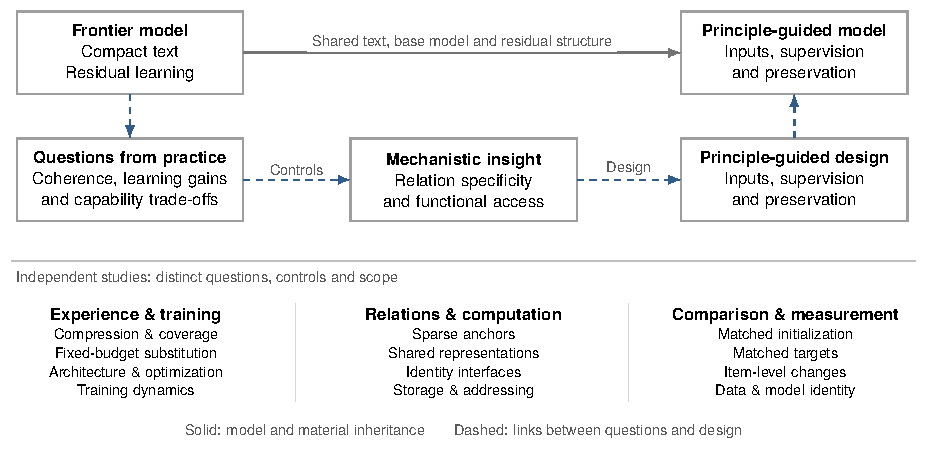
\includegraphics[width=\linewidth]{figures/research_lineage.pdf}
\caption{模型继承与研究分支。实线表示第二代模型对第一代训练文本、预训练基座和残差结构的继承；虚线表示由实践问题经机制研究形成训练设计的联系。下方归纳经验与训练、关系与计算、比较与测量三个方向的独立成果。}
\label{fig:lineage}
\end{figure}

紧凑重述首先是一种预算内的模型改进方法，随后成为可以控制表达关系的实验材料；残差增量结构首先用于成熟模型的继续学习，随后提供冻结共同基座、比较训练目标和功能保持的条件。一个有效方法因而可以同时留下模型资产和新的实验工具。第一阶段与第二阶段的联系，正体现在研究对象得到了持续使用，而解释在新的对照中不断细化。

第二阶段的两条主要分支提供互补证据。自然文本实验研究训练关系如何影响来源利用；受控绑定任务研究查询对象与属性如何对应，以及新符号能否继续使用这种计算。两类实验采用不同任务和模型，共同指向第三阶段的设计问题：让什么信息进入预测，让哪些目标获得监督，哪些已有功能需要在新学习中保持。

第三阶段把这些认识落实为三个训练操作：扩大重述侧遮盖、保留稀疏预测目标、限制普通输入上的输出偏离母模型。最终评测验证了完整方案的收益，进一步对照又区分了目标数量、输入条件和实际约束强度。图\ref{fig:lineage}分别标出模型与材料的实际继承，以及机制研究对训练设计的启发。

\subsection{经验压缩、替换与训练阶段}
\label{sec:experience_branch}

有限预算下的数据处理有两种不同作用：改变同一内容的表达方式，或者使预算能够容纳更多内容。紧凑重述将两者结合；要研究其原理，则必须分开比较。本研究形成的固定预算替换设计，把“加入什么”与“移除什么”同时作为实验条件。它适用于语料整理、数据混合和课程设计，不局限于一种重述方法。

例如，在同一 DeBERTa 配置的 80M、90M、100M 词模型上，研究比较紧凑重述、从相同来源范围选取不同句子，以及近似逐字重复。对三个训练进度的五项指标作晚期汇总后，相对参照的平均差值分别为 $+0.3853$、$+0.3350$、$+0.0343$。五项为 BLiMP、Supplement、EWoK、COMPS 与 Reading；不同句子条件扩展的是既定来源范围内的句子覆盖。改变表达和扩展内容在该配置中均有晚期收益，精确重复的作用幅度较小。

替换对象同样重要。固定加入 FineWeb 数据块，移除儿童／口语材料与移除成人散文，在 100M 处的四项均值相差 0.6125 分，前者较低；两者相对参照分别为 $+0.0825$ 与 $+0.6950$。四项只包括 BLiMP、Supplement、EWoK、COMPS。加入部分完全一样，却因移除部分不同而产生不同净收益，这是有限经验的机会成本。

另一 RoBERTa 配置中，重述方案改善了自身训练损失，晚期五项差值却为 $-0.6873$。跨配置比较由此揭示数据价值的条件性：同一类处理在不同模型和训练阶段可能产生不同效果。词频分布等文本统计可以帮助选择候选，最终判断仍来自相应任务上的实际比较。

其他压缩路线进一步区分了词面覆盖与关系完整性。抽取式紧凑视图、词汇范围受控的流畅连接文本和规则改写，分别尝试保留更多内容、补足表达衔接或减少外部生成依赖。短程比较观察到局部收益与任务代价，尚未形成相同完整度的模型结果。其可复用价值在于把压缩质量分解为可检查的条件：保留了哪些词、哪些对应关系、哪些预测线索，以及释放的预算实际去了哪里。

\subsection{关系锚点、共享表示与可识别性}
\label{sec:anchors}

有些学习困难来自信息不足以确定答案，而非训练时间不够。假如只知道几个对象分别属于相同或相反的两类，就可以恢复它们的分组，却还不知道哪一组应叫“正类”。给出少数明确标签，才能消除这个命名歧义。这类起定位作用的标签称为锚点。

研究将这一问题落实为二候选关系任务。设事件 $i$ 的关系方向为 $z_i\in\{-1,+1\}$，事件间的比较为 $r_{ij}=z_i z_j$：取值 $+1$ 表示方向相同，$-1$ 表示相反。对一组经比较相互连接的事件，整体翻转所有方向都不会改变已有比较：
\begin{equation}
 (z_i,z_j)\mapsto(-z_i,-z_j),\qquad
 (-z_i)(-z_j)=z_i z_j.
\end{equation}
一个绝对状态标签可以在这个有限假设类中确定方向。这是稀疏锚点的作用：以少量绝对信息消除仍然存在的歧义，而不是逐项重新监督全部关系。

实验让状态判断和关系比较共享同一套输入表示与序列处理网络，分别使用自己的输出层。实现采用嵌入表示（embedding）和门控循环单元（GRU）：前者将输入符号变成数值向量，后者处理序列中的联系。三个训练种子中，反转少量状态锚点后，未被直接监督的关系也随之反转，按原标签评价的准确率从 1.0 变为 0.0；而这些关系之间“相同还是相反”的判断仍全部正确。也就是说，绝对方向随锚点改变，相对关系得到保留。

变化与不变同时出现说明，少量绝对标签可以通过共享表示影响其他关系，相对结构则得到保留。使用分离表示的匹配模型可以拟合部分局部任务，却没有同样的传递。这一对照使“共享表示”从一般设计偏好变成可以检验的信息传播条件。

\begin{table}[htbp]
\caption{二值关系任务中的锚点反转。两项测量分别检验绝对方向与相对关系，报告三个训练种子的结果，准确率以 0--1 的比例表示。}
\label{tab:anchor}
\begin{tabularx}{\linewidth}{@{}Yrr@{}}
\toprule 测量对象 & 原方向 & 反转锚点后\\\midrule
未直接监督关系：按原始标签判断 & 1.0 & 0.0\\
未见关系间的相对比较准确率 & 1.0 & 1.0\\
\bottomrule
\end{tabularx}
\end{table}

这一构造说明，在给定关系结构中，哪些信息足以确定答案，以及共享表示怎样使这些信息影响其他判断；它与将对象、属性和角色建立对应的绑定表征研究相联系\citep{feng2024binding,dai2024binding}。这里已经提供候选对象和关系规则。普通文本还要求模型自行发现对象、识别表达中的关系，因此不能把一个锚点在此任务中的效果直接推广到所有语言学习。

名称与对象的匹配是关系使用的另一项前提。即使模型已能计算关系，输入名字仍需要对应到正确对象，本文将这种对应称为身份接口。字符实验提供少量表示“同一字母”的监督，使查询与候选文本的字符表示建立联系。在覆盖全部基础字母的构造中，匹配准确率从 0 提高到 1，并恢复未直接监督事件的关系响应；只覆盖部分字母或训练名字时，含未覆盖字符的新名字仍然困难。

这里的新名字由已经学习的字符组合而成。实验按位置对齐字符，给定候选对象，并在匹配器训练后固定其参数；硬分配指每次直接选定一个候选，而非混合多个候选的表示。在这些条件下，基础字符的覆盖支持了新名称组合的匹配。别名、代词及自由文本指代属于进一步的研究问题。这一结果将关系计算与输入识别分开，使“学会规则”和“识别规则应作用的对象”能够分别检验。

\subsection{实体存储、读取与语义寻址}
\label{sec:memory_branch}

显式记忆通过模型之外可读写的存储位置保存状态。要用于语言任务，系统需要从文本识别对象，将新状态写入正确位置，覆盖过时内容，再按查询读取所需状态。其中，寻址指确定应写入或读取哪个位置；语义寻址进一步要求依据文本含义作出这一选择。本研究将存储、读取与寻址分开，以定位各环节实际学会了什么。

实验先直接提供正确的写入和读取位置，称为金标准地址条件。可以把记忆槽理解为带编号的存储格：同时重新编号写入和读取位置，不应改变结果；只交换其中一个位置，则会读出不同内容。前一种操作检验结果是否不受编号方式影响，后一种操作检验模型是否真的依赖所读内容。这样便能把“信息存得住”和“模型用得上”分开研究。

将读取结果接入语言预测后，三个训练种子中正确地址条件的答案对数优势（log-odds）增益为 1.2056，定向槽交换效应为 2.0513，成对正确率为 0.0472。对数优势比较目标答案与对照答案的相对概率，成对正确率要求一对对应测试都答对。两类读数共同定位了当前能力：记忆已经影响答案概率，可靠完成成对关系判断仍是主要困难。

随后，研究用 $h+gP(m)$ 将记忆加入原表示。其中 $h$ 是模型原表示，$m$ 是读取内容，$P$ 将读取内容映射到相同维度，门控系数 $g$ 控制记忆的加入量；训练还同时降低学习率并延长学习时间。成对正确率提高至 0.1375，槽交换效应为 3.087。这是连接方式与训练设置共同调整后的结果，门控的独立贡献尚未分离。

\begin{table}[htbp]
\caption{实体记忆各环节的实验结果。不同条件分别测量存储内容的作用、地址识别、候选选择与时间状态判断。}
\label{tab:memory_layers}
\small
\begin{tabularx}{\linewidth}{@{}P{35mm}Y Y@{}}
\toprule 研究条件 & 关键观察 & 说明的功能层次\\\midrule
给定正确地址 & 槽交换改变答案概率，成对正确率仍低 & 记忆影响了预测，完整关系行为仍困难\\
从自然文本确定地址 & 总体 token 准确率 90.4\%，关键查询召回为零 & 容易位置上的高分掩盖了查询困难\\
冻结读取器、学习选择器 & 词面与角色交换约 0.994--0.995 & 给定候选中的对应选择已经可用\\
时间语义选择 & 原先／更新状态选择约 0.511 & 理解应该读取哪个时态的状态仍困难\\
\bottomrule
\end{tabularx}
\end{table}

自然文本中的困难促成了选择—读取分解：先训练出能够从指定位置读出内容的模型并将其固定，再训练另一个部分从四个候选位置中选择正确位置。后者使用 softmax 将候选得分转为概率。实验由此区分“内容读不出来”和“内容本来可读、但选错了位置”。模型能较好处理词面与角色交换，却仍难以根据时间含义判断应读取原状态还是更新状态，这进一步明确了尚需学习的内容。

任务检查还发现并排除了一项答案捷径：早期小型实体任务的正确答案不随查询对象改变，模型可依靠固定答案或首个存储位置获得高分。该结果已被撤回，不再作为组合绑定证据；修正语料本身也不构成重新训练后的验证。本章采用的是另行完成的存储、寻址与选择实验。

\subsection{优化、初始化与测量方法}
\label{sec:measurement_branch}

结构改动后的比较首先需要确认共同起点。一个删除位置相关注意力项的实验使用相同随机种子，却有 140 个共同张量中的 53 个初值不同；原因是构造顺序改变了随机数消耗。显式复制共同参数后，紧凑视图相对重复的结构交互估计从 $-0.6908$ 变为 $+0.0679$，区间跨零，而删减结构本身的绝对能力仍较低。

这一区分明确了结构比较的两个问题：删改结构后总体能力怎样变化，以及同一种数据处理在不同结构上的收益是否改变。前者仍有差异，后者原先较大的交互估计却受到初始化影响。可复用的做法是检查共同参数的名称、形状与实际初值，并显式对齐它们。

优化研究采用了类似的区分。研究通过比较不同目标要求参数改变的方向，检查它们是否互相冲突；再尝试调整冲突方向、加入检测任务或切换优化器。部分调整改善了短程损失或内部测量，却未确认稳定的完整任务收益。它们留下的认识是，更新过程看起来更协调，并不自动表示模型能力提高；是否继续投入，需要以真实任务而非仅优化器内部数值判断。

评测采用两个互补尺度。宏平均先计算各任务分数，再对任务等权平均；逐题分析则比较同一道题在训练前后是否答对。由于任务样本量不同，宏平均提高时，总答对题数仍可能下降。研究分别统计从错变对的题目、从对变错的题目及两者之差，并将 Reading 等非准确率指标单独处理。它们分别说明能力的净收益、获得与损失。

训练工程同样影响科学结论。把文本连续装入有限窗口时，研究核对完整词、来源—重述关系及截断后的实际可见内容。将大批量拆成多个微批量时，需按参与损失的目标数量加权，保持预期的平均损失。激活重计算（gradient checkpointing）通过在反向传播时重新计算部分中间结果节省显存，其数值一致性也需要检查。研究用短程、固定随机性的梯度比较检验这些实现条件；可训练参数比例、最终模型训练成本和寻找方法的研究成本则分别统计。

\subsection{研究全貌的保存方式}

以上分支形成四类可复用成果：改变真实模型的训练方法，揭示作用条件的机制实验，澄清混淆因素的测量方法，以及具有明确问题与实现的探索性构造。它们分别贡献了可运行的方法、可检验的解释、可靠的比较工具和后续研究方向。

附录\ref{app:catalog}按科学问题收录这些方法、对照和后续修正，并明确标注已有结果与待检验候选。相近方法归入共同主题，便于从问题找到操作、发现和相关章节。图表数据、模型版本与材料入口见附录\ref{app:assets}。
